%---
\section{Organization}
\label{sec:Organization}

{\bf \color{red} Definire la struttura organizzativa dell’esperimento:
\begin{itemize}
\item Spokesperson, 
\item Technical Coordinator,
\item Local Responsible,
\item Site Manager,
\item Funds Responsible,
\item GLIMO-S\&E.
\end{itemize}
}


\begin{figure*}[htbp!]
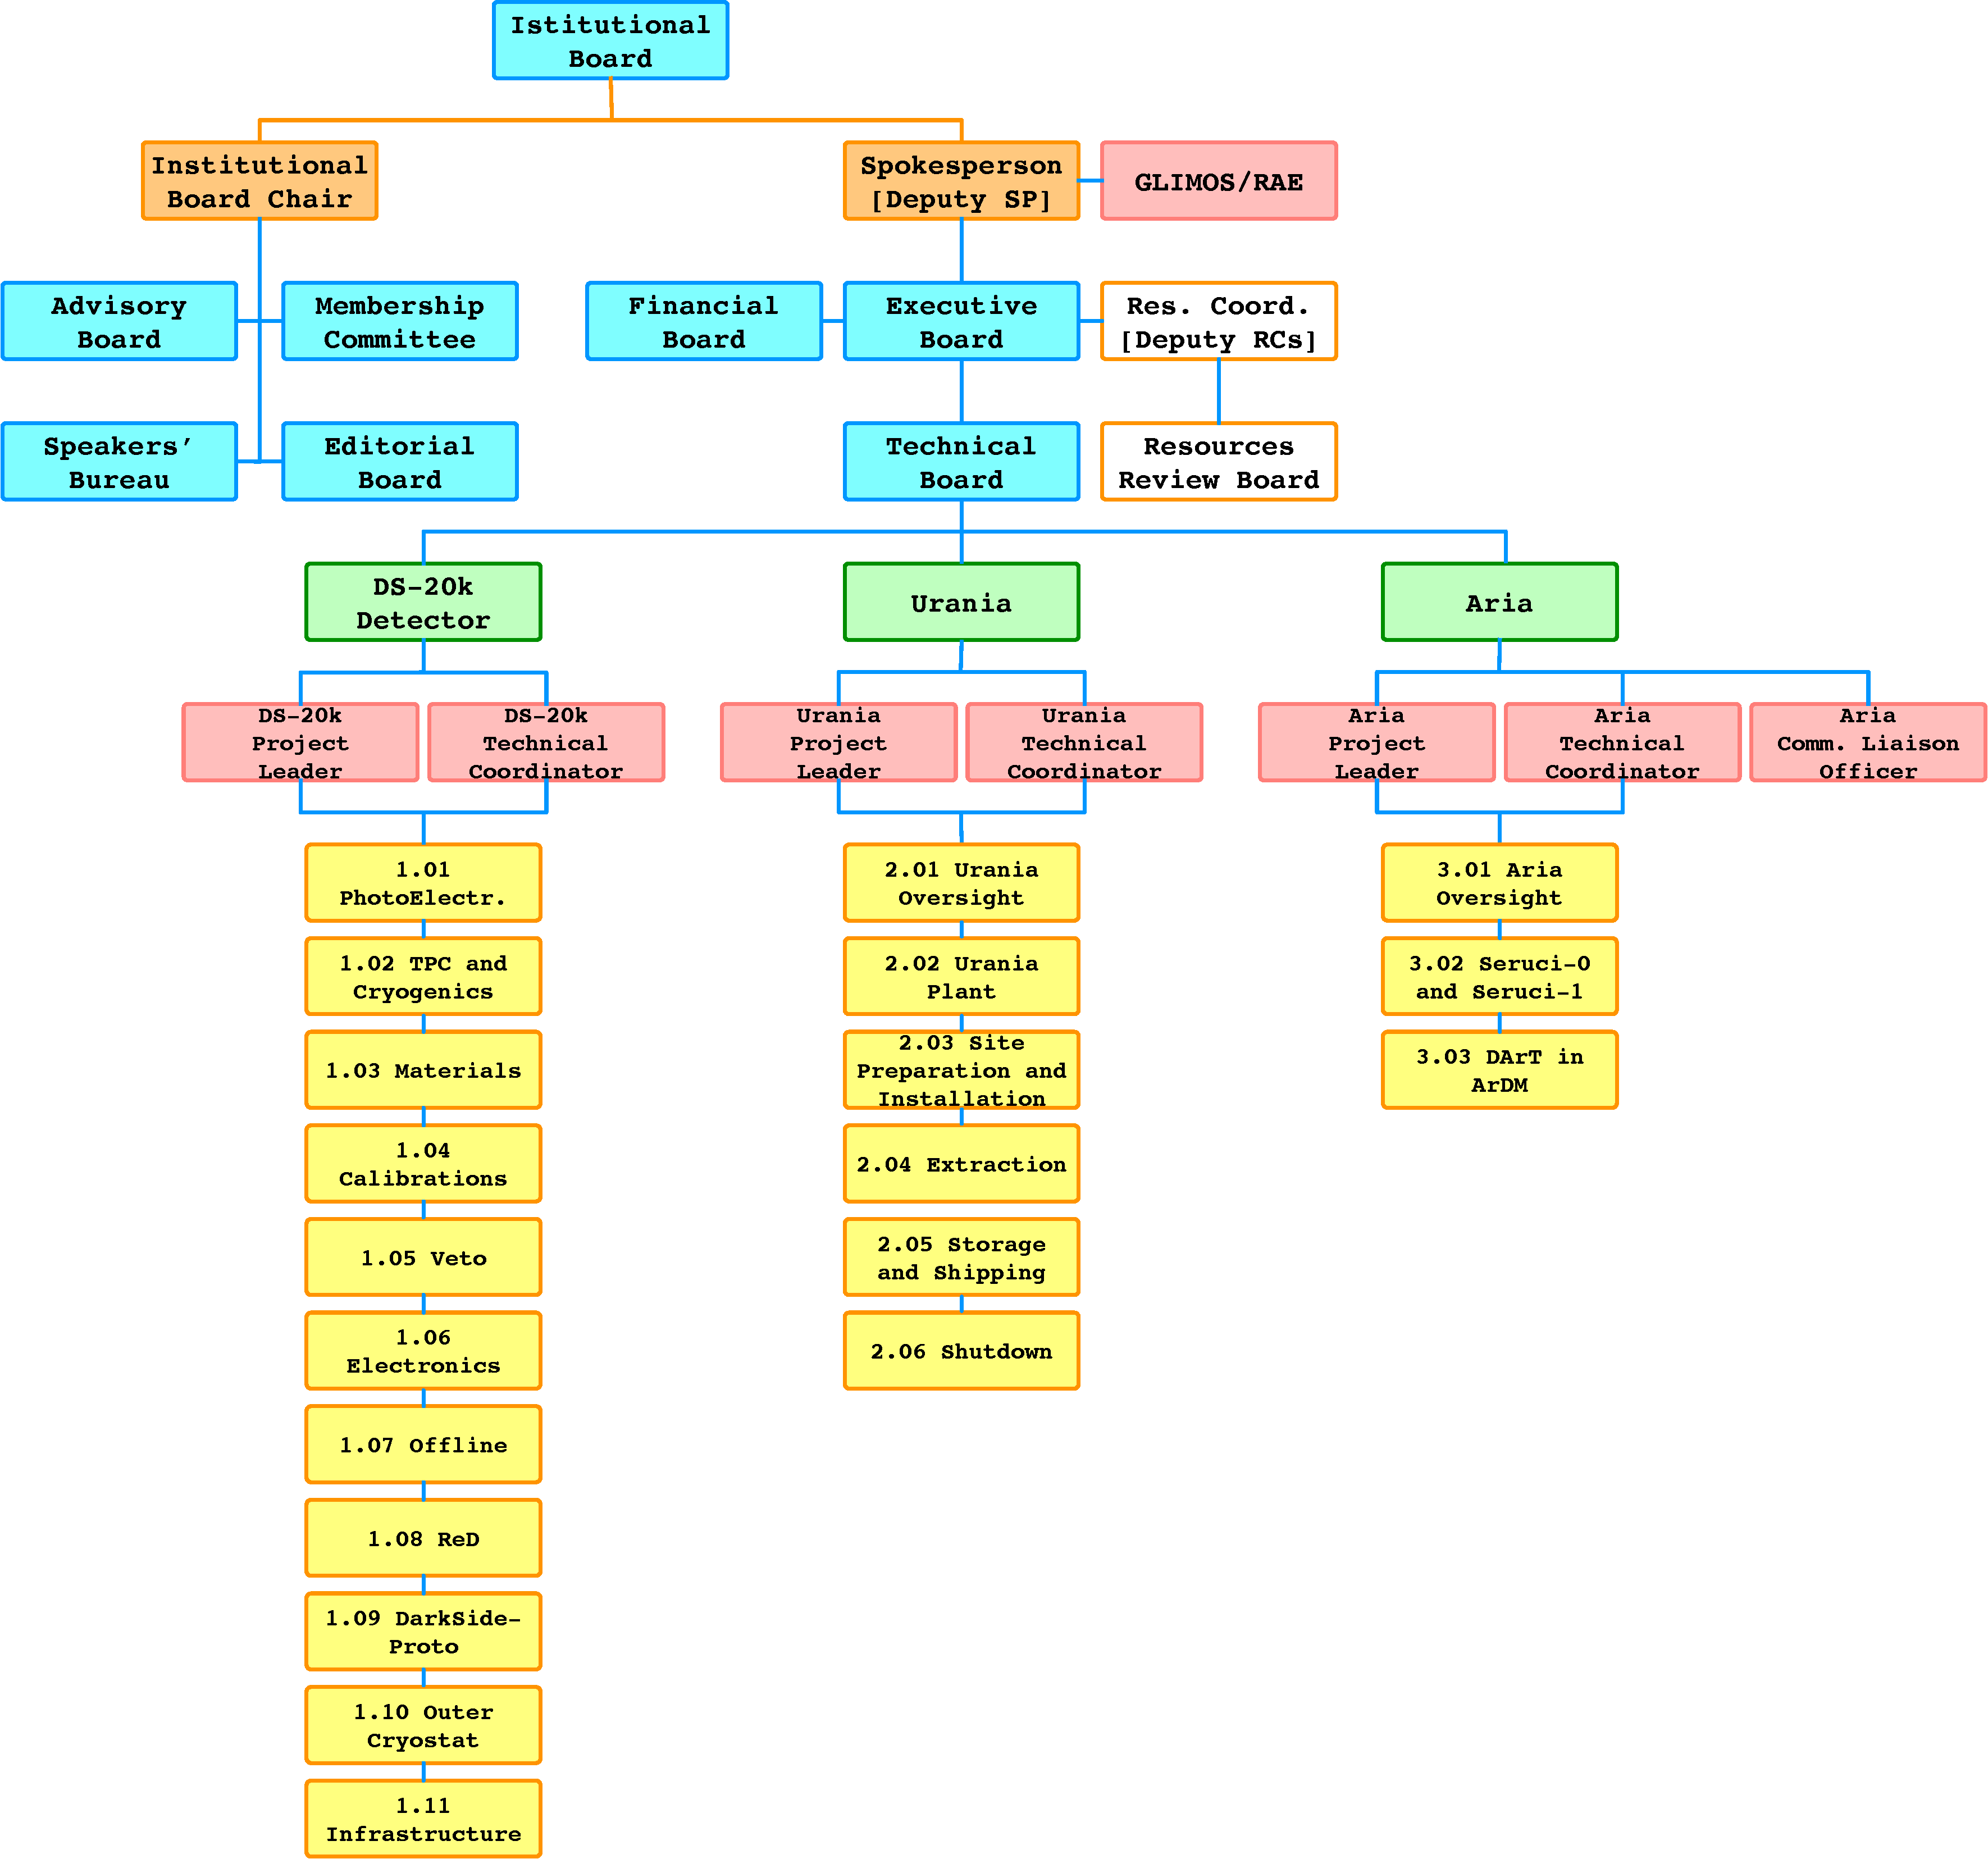
\includegraphics[width=\textwidth]{./Figures/ManagementChart.pdf}
\caption[The organization structure of the \GADMC\ and of the \DS\ project]{The organization structure of the \GADMC\ and of the \DS\ project.}
\label{fig:ManagementChart}
\end{figure*}

The organization structure of the \GADMC\ and of the \DS\ project is defined in \reffig{ManagementChart}. The governance of the \GADMC\ is carried out by two distinct branches: the policy-making branch and the executive branch.

The organization structure of the \DS\ project is defined in \reffig{ManagementChart}. The governance is carried out by two distinct branches: the policy-making branch and the executive branch.

Policy-making is done by the {\bf Institutional Board (IB)}. Each institution is represented within the IB by its PI. The IB is guided by an elected {\bf IB Chair} with a renewable \num{2}~year mandate. The IB is responsible for the definition of rules and the governance of the Collaboration, the overall organization of the Collaboration, the appointment of all managers belonging to the policy-making and executive branches; the final approval of major design changes proposed by the executive branch; and the control of financial and human resources.  The current IB Chair is G.~Batignani (Pisa), elected in November~2016 and re-confirmed in November~2018.

Within the policy-making branch there are three committees charged with providing recommendations to the IB and its Chair.  The members of the three committees are appointed by the IB upon proposal of the IB Chair, taking into account the composition of the Collaboration and the need to represent its diverse composition.  These three committees are:

\begin{compactitem}
\item[\bf The Advisory Board,] consisting of the IB Chair and \num{6}~senior IB members nominated by the IB Chair, of which \num{2}~members are from Italian institutions, \num{1}~member is from a US institution, \num{1}~member is from a Canadian institution, and \num{2}~members are from institutions outside the three countries already listed.  This committee is mandated with advising the IB Chair on IB management issues.
\item[\bf The Membership Committee,] consisting of \num{6}~members nominated by the Advisory Board and confirmed by the IB, as well as \num{2} {\it ex officio} Advisory Board members.  This committee addresses requests from new groups wishing to join the Collaboration, helps define the commitments of new groups, and maintains the database and mailing lists of the collaboration.
\end{compactitem}
\smallskip
There are two additional committees within the policy-making branch charged with providing recommendations to the IB on the communication of scientific and technological results.  The members of the two committees are appointed by the IB upon proposal of the IB Chair, taking into account the composition of the Collaboration and the need to represent its diverse composition.  The two committees are:

\begin{compactenum}
\item[\bf The Speakers' Bureau,] consisting of \num{5}~members nominated by the Advisory Board and confirmed by the IB, \num{1} {\it ex officio} Advisory Board member, and the SP and Deputy SP.  This committee appoints speakers at conferences and workshops and approves material that will be presented on behalf of the Collaboration.
\item[\bf The Editorial Board,] consisting of \num{6}~members nominated by the Advisory Board and confirmed by the IB.  This committee approves the start of paper preparation, guides the internal paper review process, and issues final approval of papers before publication.
\end{compactenum}

The executive branch of the \GADMC\ is led by an elected {\bf Spokesperson (SP)}.  The primary responsibility of the SP is to oversee the \DSks\ experiment, oversee any other scientific efforts pursued by the Collaboration, and act as the Collaboration's primary public face.  The SP is assisted by an elected {\bf Deputy SP (dSP)}.  The mandates of the SP and dSP are \num{3}~years, renewable.  C.~Galbiati and G.~Fiorillo were elected as SP and Deputy SP respectively in December 2016.

The \DSk\ project is organized into \num{3} sub-projects: {\bf the \DSks\ detector}, {\bf \Urania}, and {\bf \Aria}. Each of the sub-projects is managed by two {\bf Project Coordinators (PCs)}, {\it i.e.}, a {\bf Project Leader (PL)} and a {\bf Technical Coordinator (TC)}.  The PL manages the overall progress of the sub-project and is responsible for and coordinates the {\bf Level-1 (L1) Work Groups (WGs)} in which the sub-project tasks and objectives are subdivided and organized, ensuring that the design and construction of the sub-project is carried out on schedule, within the cost ceiling, and in a way that meets the performance and reliability requirements determined within the framework of \GADMC\ resource planning.  The PL plans the schedule and budget, sets deadlines, and monitors quality and progress of the sub-project under their oversight.  The TC is responsible for the sub-project construction and the technical integration of all its components. The TC ensures the implementation of engineering standards and procedures, monitors the overall construction of detectors and infrastructure, and is responsible for the sub-project's integration and safety. The \Aria\ sub-project, due to its complex nature, has an additional PC, a {\bf Community Liaison Officer} charged to act as a link with the local authorities in Sardinia.

In addition to the PCs defined above, three {\bf Project Scientists (PSs)} are charged with the scientific oversight of the detector design and construction to ensure that all technical decisions are fully compliant with the requirements of the project and compatible across all sub-systems.

The management of each sub-project is divided between {\bf Level-1 (L1) Managers} and {\bf Level-2 (L2) Managers}, who are responsible for the direction of the {\bf L1} and {\bf L2 WGs} in which the sub-project are organized and structured.

The {\bf Executive Board (EB)}, which is chaired by the SP and includes as members the dSP, the PSs, all PCs, and all L1 Managers, manages the executive branch of the \GADMC.  The IB Chair is an {\it ex officio} member of the EB.  The SP regularly invites senior PIs charged with significant organization and funding responsibilities but without a formal PC role to the EB meetings.

The PSs and the PCs of \DSks\ and \Urania\ report to the EB.  The PCs of \Aria\ report to the {\bf Scientific Responsible (SR) of \Aria}, which is jointly appointed by \INFN\ and the Regione Autonoma della Sardegna.  The SR of \Aria\ is C.~Galbiati, the inventor and founder of the \Aria\ program.  The SR of \Aria\ reports to the EB.

All PCs and PSs are nominated by the SP to the EB, proposed by the EB to the IB, and appointed by the IB.  PCs are required to pledge that \DSks\ will be their top scientific priority and that they will dedicate a dominant fraction of their research time to their effort within the \GADMC.  The EB and by the IB monitor closely the effectiveness of the PCs.

The L1 Managers are proposed by the PCs, confirmed by the EB, and appointed by the IB.  The L1 Managers report to the PCs.  The L2 Managers are proposed by the L1 coordinators in concurrence with the PCs, confirmed by the EB, and appointed by the IB.  The L2 Managers report to the L1 Managers.

The {\bf Technical Board (TB)}, chaired by the SP and with a membership of the dSP, the PSs, all PCs, and all L1 and L2 Managers, is responsible for the execution of the project.  The IB Chair is an {\it ex officio} member of the TB.  All TB meetings and calls are open to the entire Collaboration.  The TB is the forum where all major and minor decisions affecting the project are debated and finalized.  In its decision making process, the TB typically operates by building consensus.  The TB also monitors the execution of the individual sub-projects and discusses matters at the interface between different sub-projects.  All TB meetings are prepared and chaired by the \DSks\ TC.

The \DS\ resource coordination is delegated to a {\bf Resources Coordinator (RC)}, who has responsibility for the administration of the common fund.  The RC is appointed by the IB upon proposal of the EB.
  
The {\bf Resources Review Board (RRB)} is made up of representatives from the funding agencies providing major contributions to the project, the IB Chair, the SP, the dSP, the RC, and the {\bf Country Representatives (CRs)}, who are appointed by the assembly of PIs supported by any given funding agency and is in charge of the relationship with said agency. The RRB responsibilities include the monitoring and management of the financial instruments that constitute the \GADMC\ resources, defining the national and regional contributions to the project, developing the MoU, and approving in-kind contributions.  The {\bf Financial Board (FB)} is composed of the {\bf CRs} and advises the SP on the specific allocation of tasks and funding requests.

A requirement of the \LNGS\ Safety Management System is the appointment of a collaborator as a {\bf Group Leader in Matters of Safety (GLIMOS)}. The GLIMOS has the primary responsibility for health and safety within the Collaboration, providing an interface with \LNGS.  The GLIMOS is appointed by the \LNGS\ Director upon recommendation by the Collaboration.  An additional requirement of the \LNGS\ Environmental Management System is the appointment of a collaborator as contact person for environmental issues or {\bf Referente Ambientale dell'Esperimento (RAE)}.  The RAE acts as the link between the experimental collaboration and \LNGS\ for all matters concerning environmental protection.  The RAE is appointed by the \LNGS\ Director upon recommendation by the Collaboration management

%---
\subsection{Specific Roles and Responsibilities}
\label{sec:Organization-RolesResponsibilities}

\reftab{ManagerialRoles} offers a brief summary of the most significant executive responsibilities within the 3 sub-projects.

\begin{table}[t]
\begin{center}
%\resizebox{\textwidth}{!}{
\begin{tabular}{cccc}
\hline
\hline
\multirow{3}{*}{{\bf Project Scientists}}
						&\multirow{3}{*}{}					&P.~Meyers			&Princeton\\
						&									&W.~Bonivento		&\INFN\ Cagliari\\
						&									&A.~Razeto			&\INFN\ \LNGS\\
\hline
\multirow{2}{*}{{\bf \DSks\ Project Coordinators}}
						&Project Leader						&E. Scapparone		&\INFN\ Bologna\\
						&Technical Coordinator				&An.~Ianni			&Princeton\\
\hline
\multirow{14}{*}{{\bf \DSks\ L1 Managers}}
						&\DSp\ Managers						&G.~Fiorillo		&\INFN\ Napoli\\
						&Technical Integration Manager		&T.~Napolitano 		&\INFN\ LNF\\
						&Materials Manager					&R.~Santorelli		&CIEMAT\\
						&\ArDM\ Manager						&C.~Regenfus		&ETH Z\"urich\\
						&Inner Detector Manager				&H.~Wang			&UCLA\\
						&Deputy Inner Detector Manager		&E.~Pantic			&UC Davis\\	
						&Outer Detector Manager				&G.~Testera 		&\INFN\ Genova\\			
						&Deputy Outer Detector Manager		&J.~Monroe			&RHUL\\	
						&PhotoElectronics Manager			&A.~Razeto			&\INFN\ \LNGS\\
						&Electronics Manager				&M.~Rescigno		&\INFN\ Roma 1\\
						&Calibration Manager				&J.~Maricic			&Hawai'i\\
						&Offline Manager					&D.~Franco			&CNRS/IN2P3\\
						&\ReD\ Manager						&L.~Pandola 		&\INFN\ \LNS\\
						&Outer Cryostat Manager				&M.~Nessi			&\CERN\\
\hline
\multirow{2}{*}{{\bf \Urania\ Project Coordinators}}
						&Project Leader						&M.~Simeone			&\INFN\ Napoli\\
						&Technical Coordinator				&A.~Renshaw 		&University of Houston\\
\hline
\multirow{3}{*}{{\bf \Urania\ L1 Managers}}
						&Plant Manager						&M.~Simeone 		&\INFN\ Napoli\\
						&Site Preparation and Installation	&A.~Renshaw			&Houston\\
						&Extraction							&H.~Back			&\PNNL\\
\hline
\multirow{5}{*}{{\bf \Aria\ Project Coordinators}}
						&Project Leader						&W.~Bonivento		&\INFN\ Cagliari\\
						&Deputy Project Leader				&F.~Gabriele 		&\INFN\ \LNGS\\
						&Technical Coordinator				&R.~Tartaglia 		&\INFN\ \LNGS\\
						&Deputy Technical Coordinator		&M.~Razeti			&\INFN\ Cagliari\\
						&Community Liason Officer			&A.~Devoto			&\INFN\ Cagliari\\
\hline
\multirow{2}{*}{{\bf \Aria\ L1 Managers}}
						&\SeruciOne\ Manager				&F.~Gabriele 		&\INFN\ \LNGS\\
						&\DArT\ Manager						&W.~Bonivento		&\INFN\ Cagliari\\
\hline
\end{tabular}%}
\caption[Managerial roles of the project]{Overview of the most significant managerial roles within the \DS\ sub-projects.}
\label{tab:ManagerialRoles}
\end{center}
\end{table}

%%---
%\subsection{Partnerships}
%% that is capable of collecting a \ArgoExposure\ exposure while eliminating all backgrounds beyond \NR\ events induced by atmospheric and diffuse supernova background neutrinos. These scientists also agreed to form the Global Argon Dark Matter Collaboration (\GADMC), a consortium of institutes active in the development of argon dark matter experiments.  
%
%The Global Argon Dark Matter Collaboration (\GADMC) is composed of scientists from four \LAr\ dark matter projects (\ArDM\ at \LSC, \DSfs\ at LNGS, and \DEAP\ and \mCLEAN\ at \SNOLAB) who have agreed to unify efforts and construct \DSk\ at \LNGS~\cite{Boulay:2017tn}. These same scientists have signed a Letter of Intent signaling their interest in continuing the collaboration beyond \DSks\ to build a \LAr\ detector with a several hundred tonne fiducial mass. The \GADMC\ will oversee the open access of the currently operating \LAr\ dark matter experiments (\DSfs\ and \DEAP) and scientific data to all \GADMC\ institutions, coordinate the construction of \DSks\ at \LNGS, and coordinate the development of a future \LAr\ dark matter detector with a several hundred tonne fiducial mass.
%
%The \GADMC\ collaboration is currently composed of \num{59} institutions and \num{371} scientists from 15 nations: Brazil, Canada, China, France, Germany, Greece, Italy, Mexico, Poland, Romania, Russia, Spain, Switzerland, the United Kingdom, and the United States of America.
%
%\DSks\ was jointly proposed to the US \NSF, the Italian \INFN, and \LNGS, the host laboratory, in December~2015.  The experiment was first reviewed by a joint panel charged by the Italian \INFN\ and the US \NSF.  The joint review was made possible by NSF statute NSF-14-1999 ``Dear Colleague Letter - International Activities within the Physics Division - Potential International Co-Review''~\cite{USNationalScienceFoundation:2014vy} following approval by the US State Department.  Following the first joint review, the experiment was also reviewed by the \INFN\ {\it Commissione Scientifica Nazionale Seconda} (CSN2), the \INFN\ {\it Comitato Tecnico Scientifico} (CTS),  the \LNGS\ Scientific Committee, and the ``Particle Astrophysics -- Experiment'' panel of \NSF.  Following all reviews, the experiment was approved by \INFN\ and \LNGS\ in April~2017 and by \NSF\ in October~2017.  Following a meeting of participating international funding agencies and laboratories held at the Embassy of Canada in Rome in September~2017, the experiment was officially supported by three participating underground laboratories: the host laboratory \LNGS, Laboratorio Subterr\'aneo de Canfranc (\LSC), and \SNOLAB.  Future reviews of the experiment's progress may also involve a coordinated effort by the Directorates of the three laboratories.
%
%\INFN\ has provided most of the capital funds needed to support the \DSks\ project. R\&D and laboratory set-up costs have been covered by INFN CSN2. Additional funding in Italy, including support for the \Urania, \Aria, and \NOA\ facilities, comes from special and regional funds, the Ministero dello Sviluppo Economico (MISE), the Ministero dell'Istruzione, from the Universita e Ricerca (MIUR), the Regione Abruzzo, and the Regione Autonoma della Sardegna.  The Regione Autonoma della Sardegna and INFN instituted a Comitato di Indirizzo to manage the Aria project.  The Regione Autonoma della Sardegna and \INFN\ instituted a {\it Comitato di Indirizzo} to oversee and monitor the \Aria\ project.
%
%Several groups from Canada joined the Collaboration in September~2017. They have secured funding for the large scale extraction of low-radioactivity argon from \CFI\ in Canada and funding for \DEAP\ R\&D from \NSERC.  An internal proposal for capital funds to support \DSks\ activities was submitted to \TRIUMF\ in October~2017 and was approved for funding.  A proposal to the Canadian \CFI\ for additional capital funds will be submitted October 2019.
%
%University groups from Poland, Russia, Spain, and Switzerland are funded to work on \DSks\ by their funding agencies.  University groups from France, Germany, and the UK are currently participating with support from internal resources and are preparing proposals to each of their funding agencies.
%
%Recently, \INFN\ and The Institute of High Energy Physics of the Chinese Academy of Sciences (\IHEP) reached an agreement to produce the acrylic material for both the \TPC\ and the veto detectors in China.  The production will be carried out by DonChamp, Inc. in Changzhou, the same company providing acrylic for the \JUNO\ experiment.  The \IHEP\ group submitted a request for capital funding to the Chinese Ministry of Science to support the acquisition of the \PMMA\ for the the veto detector and the \LArTPC.
%
%The \DSks\ experiment is hosted by \LNGS.  The \LNGS\ Scientific Committee, which meets two times per year, has oversight of the experiment and has assigned two Committee members as reviewers of \DSks.  The reviewers evaluate technical developments, schedule compliance, and collaboration issues, and report their findings to the \LNGS\ Scientific Committee.  The \LNGS\ Scientific Committee regularly requests that the \GADMC\ provide a written report from the collaboration two weeks before its meetings and present technical results during the meetings' open session, and that the Collaboration management be available for discussion in its closed sessions.  The \LNGS\ Scientific Committee issues a report with its findings after each meeting, which details the progress of the Collaboration and offers recommendations.  The \GADMC\ is also requested to release an annual document to \LNGS\ for inclusion in the {\em LNGS Annual Report}.
%
%Within \INFN, the experiment is regularly reviewed by the CSN2, which oversees technical developments and budget, collaboration, and schedule issues.  CSN2 appoints six permanent referees charged with the review and monitoring of \DSks.  CSN2 meets every second month and on average deals with \DSks\ matters in its plenary session twice per year.  
%
%A strong connection between the \DSks\ funding agencies is fostered through ad-hoc meetings between the \INFN\ management and the management of other funding agencies, including the US \NSF, the US \DOE, the Chinese \IHEP, the French \INDPT, and \CERN. In addition, the \DSk\ management has organized six meetings at the Canadian Embassies of Italy, France, Spain, Mexico, and Poland, and at the Italian Consulate in Montreal, Canada.  The six meetings celebrated the Nobel Prize in Physics awarded to Prof. Art McDonald, who is a founding member of the \GADMC\ and an active participant in \DSks, and took the opportunity to present to a broad audience, which included agency officials and government representatives, the short- and long-term plans of the \GADMC.
%
%
%%---
%\subsection{External Organization and Communication}
%
%The Spokesperson is responsible for external communications.  Relationships with the funding agencies are maintained by the Country Representatives and by the Spokesperson.
%
%
%%---
%\subsection{Institutional Responsibilities}
%
%The assignment of tasks and responsibilities to the various collaborating institutions is captured in a Primavera P6-based resource-loaded work breakdown structure (WBS) managed by the \DSks\ TC and by the project controls team. The WBS is presented in schematic form in \reffig{WBS} and a summary of the institutional participation by task is summarized in \reftab{InstitutionalResponsibilities}.
%
%\begin{table}[t]
%\begin{center}
%\begin{tabular}{lc}
%\hline
%\hline
%\multirow{1}{*}{{\bf Outer cryostat}} 				&\INFN\ (L), \CERN,	UCLA, Princeton\\
%\hline
%\multirow{1}{*}{{\bf Inner detector}} 				&UCLA (L), \FNAL, UMass, \INFN, Alberta, Carleton, Queens, Houston, UC Davis\\
%\hline
%\multirow{1}{*}{{\bf Photoelectronics}} 			&\INFN\ (L), \GSSI, UMass, Princeton\\ 
%\hline
%\multirow{1}{*}{{\bf Outer detector}}				&Genova (L), \LNGS, AstroCeNT, Virginia Tech, Royal Holloway, \IHEP\\
%\hline
%\multirow{1}{*}{{\bf Calibration}}					&Hawai'i (L), Temple, Princeton, BNRU/RSU, Virginia Tech, Krakow, \LNGS, \LNF\\
%\hline
%\multirow{1}{*}{{\bf Electronics}}					&\INFN\ (L), \CERN, \TRIUMF\\
%\hline
%\multirow{1}{*}{{\bf Online\&Offline SW}} 			&APC Paris (L), \INFN, LPNHE, Paris\\ 		
%\hline
%\multirow{1}{*}{{\bf Material screening}} 			&CIEMAT (L), \SNOLAB, Krakow, \INFN, \LSC, LNL, Zaragoza\\
%\hline
%\multirow{1}{*}{{\bf \ReD}}	 						&\INFN\ (L), APC, LNS, USP\\
%\hline
%\multirow{1}{*}{{\bf \DSps}}						&\INFN\ (L),  most \GADMC\ institutions\\
%\hline
%\multirow{1}{*}{{\bf \Urania }} 					&\INFN\ (L), Houston (L), UMass, \PNNL, Carleton\\											
%\hline
%\multirow{1}{*}{{\bf \Aria }} 						&\INFN\ (L), Princeton, \FNAL, \CERN\\	
%\hline
%\multirow{1}{*}{{\bf \DArT }} 						&\LSC\ (L), ETHZ, CIEMAT, APC, Carleton, Zaragoza\\		
%\hline
%\end{tabular}%}
%\caption[Breakdown of institutional responsibilities]{Breakdown of institutional responsibilities. Lead institutions are marked with (L).}
%\label{tab:InstitutionalResponsibilities}
%\end{center}
%\end{table}
%
%%---
%\subsection{Partnerships}
%% that is capable of collecting a \ArgoExposure\ exposure while eliminating all backgrounds beyond \NR\ events induced by atmospheric and diffuse supernova background neutrinos. These scientists also agreed to form the Global Argon Dark Matter Collaboration (\GADMC), a consortium of institutes active in the development of argon dark matter experiments.  
%
%The Global Argon Dark Matter Collaboration (\GADMC) is composed of scientists from four \LAr\ dark matter projects (\ArDM\ at \LSC, \DSfs\ at LNGS, and \DEAP\ and \mCLEAN\ at \SNOLAB) who have agreed to unify efforts and construct \DSk\ at \LNGS~\cite{Boulay:2017tn}. These same scientists have signed a Letter of Intent signaling their interest in continuing the collaboration beyond \DSks\ to build a \LAr\ detector with a several hundred tonne fiducial mass. The \GADMC\ will oversee the open access of the currently operating \LAr\ dark matter experiments (\DSfs\ and \DEAP) and scientific data to all \GADMC\ institutions, coordinate the construction of \DSks\ at \LNGS, and coordinate the development of a future \LAr\ dark matter detector with a several hundred tonne fiducial mass.
%
%The \GADMC\ collaboration is currently composed of \num{59} institutions and \num{371} scientists from 15 nations: Brazil, Canada, China, France, Germany, Greece, Italy, Mexico, Poland, Romania, Russia, Spain, Switzerland, the United Kingdom, and the United States of America.
%
%\DSks\ was jointly proposed to the US \NSF, the Italian \INFN, and \LNGS, the host laboratory, in December~2015.  The experiment was first reviewed by a joint panel charged by the Italian \INFN\ and the US \NSF.  The joint review was made possible by NSF statute NSF-14-1999 ``Dear Colleague Letter - International Activities within the Physics Division - Potential International Co-Review''~\cite{USNationalScienceFoundation:2014vy} following approval by the US State Department.  Following the first joint review, the experiment was also reviewed by the \INFN\ {\it Commissione Scientifica Nazionale Seconda} (CSN2), the \INFN\ {\it Comitato Tecnico Scientifico} (CTS),  the \LNGS\ Scientific Committee, and the ``Particle Astrophysics -- Experiment'' panel of \NSF.  Following all reviews, the experiment was approved by \INFN\ and \LNGS\ in April~2017 and by \NSF\ in October~2017.  Following a meeting of participating international funding agencies and laboratories held at the Embassy of Canada in Rome in September~2017, the experiment was officially supported by three participating underground laboratories: the host laboratory \LNGS, Laboratorio Subterr\'aneo de Canfranc (\LSC), and \SNOLAB.  Future reviews of the experiment's progress may also involve a coordinated effort by the Directorates of the three laboratories.
%
%\INFN\ has provided most of the capital funds needed to support the \DSks\ project. R\&D and laboratory set-up costs have been covered by INFN CSN2. Additional funding in Italy, including support for the \Urania, \Aria, and \NOA\ facilities, comes from special and regional funds, the Ministero dello Sviluppo Economico (MISE), the Ministero dell'Istruzione, from the Universita e Ricerca (MIUR), the Regione Abruzzo, and the Regione Autonoma della Sardegna.  The Regione Autonoma della Sardegna and INFN instituted a Comitato di Indirizzo to manage the Aria project.  The Regione Autonoma della Sardegna and \INFN\ instituted a {\it Comitato di Indirizzo} to oversee and monitor the \Aria\ project.
%
%Several groups from Canada joined the Collaboration in September~2017. They have secured funding for the large scale extraction of low-radioactivity argon from \CFI\ in Canada and funding for \DEAP\ R\&D from \NSERC.  An internal proposal for capital funds to support \DSks\ activities was submitted to \TRIUMF\ in October~2017 and was approved for funding.  A proposal to the Canadian \CFI\ for additional capital funds will be submitted October 2019.
%
%University groups from Poland, Russia, Spain, and Switzerland are funded to work on \DSks\ by their funding agencies.  University groups from France, Germany, and the UK are currently participating with support from internal resources and are preparing proposals to each of their funding agencies.
%
%Recently, \INFN\ and The Institute of High Energy Physics of the Chinese Academy of Sciences (\IHEP) reached an agreement to produce the acrylic material for both the \TPC\ and the veto detectors in China.  The production will be carried out by DonChamp, Inc. in Changzhou, the same company providing acrylic for the \JUNO\ experiment.  The \IHEP\ group submitted a request for capital funding to the Chinese Ministry of Science to support the acquisition of the \PMMA\ for the the veto detector and the \LArTPC.
%
%The \DSks\ experiment is hosted by \LNGS.  The \LNGS\ Scientific Committee, which meets two times per year, has oversight of the experiment and has assigned two Committee members as reviewers of \DSks.  The reviewers evaluate technical developments, schedule compliance, and collaboration issues, and report their findings to the \LNGS\ Scientific Committee.  The \LNGS\ Scientific Committee regularly requests that the \GADMC\ provide a written report from the collaboration two weeks before its meetings and present technical results during the meetings' open session, and that the Collaboration management be available for discussion in its closed sessions.  The \LNGS\ Scientific Committee issues a report with its findings after each meeting, which details the progress of the Collaboration and offers recommendations.  The \GADMC\ is also requested to release an annual document to \LNGS\ for inclusion in the {\em LNGS Annual Report}.
%
%Within \INFN, the experiment is regularly reviewed by the CSN2, which oversees technical developments and budget, collaboration, and schedule issues.  CSN2 appoints six permanent referees charged with the review and monitoring of \DSks.  CSN2 meets every second month and on average deals with \DSks\ matters in its plenary session twice per year.  
%
%A strong connection between the \DSks\ funding agencies is fostered through ad-hoc meetings between the \INFN\ management and the management of other funding agencies, including the US \NSF, the US \DOE, the Chinese \IHEP, the French \INDPT, and \CERN. In addition, the \DSk\ management has organized six meetings at the Canadian Embassies of Italy, France, Spain, Mexico, and Poland, and at the Italian Consulate in Montreal, Canada.  The six meetings celebrated the Nobel Prize in Physics awarded to Prof. Art McDonald, who is a founding member of the \GADMC\ and an active participant in \DSks, and took the opportunity to present to a broad audience, which included agency officials and government representatives, the short- and long-term plans of the \GADMC.
%
%
%%---
%\subsection{External Organization and Communication}
%
%The Spokesperson is responsible for external communications.  Relationships with the funding agencies are maintained by the Country Representatives and by the Spokesperson.
%
%
%%---
%\subsection{Institutional Responsibilities}
%
%The assignment of tasks and responsibilities to the various collaborating institutions is captured in a Primavera P6-based resource-loaded work breakdown structure (WBS) managed by the \DSks\ TC and by the project controls team. The WBS is presented in schematic form in \reffig{WBS} and a summary of the institutional participation by task is summarized in \reftab{InstitutionalResponsibilities}.
%
%\begin{table}[t]
%\begin{center}
%\begin{tabular}{lc}
%\hline
%\hline
%\multirow{1}{*}{{\bf Outer cryostat}} 				&\INFN\ (L), \CERN,	UCLA, Princeton\\
%\hline
%\multirow{1}{*}{{\bf Inner detector}} 				&UCLA (L), \FNAL, UMass, \INFN, Alberta, Carleton, Queens, Houston, UC Davis\\
%\hline
%\multirow{1}{*}{{\bf Photoelectronics}} 			&\INFN\ (L), \GSSI, UMass, Princeton\\ 
%\hline
%\multirow{1}{*}{{\bf Outer detector}}				&Genova (L), \LNGS, AstroCeNT, Virginia Tech, Royal Holloway, \IHEP\\
%\hline
%\multirow{1}{*}{{\bf Calibration}}					&Hawai'i (L), Temple, Princeton, BNRU/RSU, Virginia Tech, Krakow, \LNGS, \LNF\\
%\hline
%\multirow{1}{*}{{\bf Electronics}}					&\INFN\ (L), \CERN, \TRIUMF\\
%\hline
%\multirow{1}{*}{{\bf Online\&Offline SW}} 			&APC Paris (L), \INFN, LPNHE, Paris\\ 		
%\hline
%\multirow{1}{*}{{\bf Material screening}} 			&CIEMAT (L), \SNOLAB, Krakow, \INFN, \LSC, LNL, Zaragoza\\
%\hline
%\multirow{1}{*}{{\bf \ReD}}	 						&\INFN\ (L), APC, LNS, USP\\
%\hline
%\multirow{1}{*}{{\bf \DSps}}						&\INFN\ (L),  most \GADMC\ institutions\\
%\hline
%\multirow{1}{*}{{\bf \Urania }} 					&\INFN\ (L), Houston (L), UMass, \PNNL, Carleton\\											
%\hline
%\multirow{1}{*}{{\bf \Aria }} 						&\INFN\ (L), Princeton, \FNAL, \CERN\\	
%\hline
%\multirow{1}{*}{{\bf \DArT }} 						&\LSC\ (L), ETHZ, CIEMAT, APC, Carleton, Zaragoza\\		
%\hline
%\end{tabular}%}
%\caption[Breakdown of institutional responsibilities]{Breakdown of institutional responsibilities. Lead institutions are marked with (L).}
%\label{tab:InstitutionalResponsibilities}
%\end{center}
%\end{table}
%
%%The outer cryostat task is managed by \CERN\ and \INFN\ and has active participation from UCLA (cryogenic system) and Princeton. 
%
%%The inner detector task is led by UCLA (overall design and cryogenic system) with  contributions from \FNAL\ (cryogenics); Roma1 (test facility); Alberta, Carleton and Queens (machining and assembly of the acrylic parts, TPB coating); Napoli (intergration), Houston (extraction grid); and UC Davis (HV system, field and reflector cage). 
%
%%The photoelectronics task is led by \INFN\ with contributions from Bologna (overall coordination, motherboards, \NOA\ coordination, optical link), \GSSI\ and \LNGS\ (overall system design, front end electronics and tests, optical link), Cagliari (optical link), Pisa (PDMs), Genova and  Naples (testing), Princeton (\SiPM\ packaging), and Milano (cabling). 
%
%%The DAQ task is led by Roma1 with contributions from TRIUMF (readout boards and software) and \LNGS\ (infrastructure and power supply). 
%
%%The outer detector task is led by Genova with contributions from \LNGS\ (\TPB\ evaporation), AstroCeNT (reflectors), Royal Holloway (simulation), and \IHEP\ (\PMMA\ and \ce{Gd}-loaded \PMMA).
%
%%The calibration task is led by Hawaii with contributions from Temple (deployment of external systems); Princeton, BNRU/RSU, Virginia Tech and Krakow (source procurement); and Princeton, \LNGS, and LNF (on-site installation).
%
%%The online and offline software task is led by APC Paris with important contributions from Roma1 (offline software) and LPNHE Paris.
%
%%The Material screening task is led by CIEMAT with materials screenings performed  at \SNOLAB, Krakow, \LNGS\ and \LSC, with additional contributions from LNL (copper cleaning) and Zaragoza (cosmogenic activation studies). 
%
%%The \ReD\ calibration is experiment is led by \INFN\ with contributions from APC, Napoli, Cagliari, Genova, Roma1, LNGS, LNS, Roma3, and USP.
%
%%The \DSps\ effort is led by  Napoli but is a collaborative effort including most of the \DSk\ institutions.
%
%%\Urania\ is led by Napoli (plant design) and Houston (site preparation and installation), and has very important contributions from BNL and PNNL (extraction), as well as Carleton (storage and shipping). 
%
%%\Aria\ is led by \INFN\ with important contributions from Princeton (design and coordination), Cagliari (overall coordination and contact with local authorities) and has important contributions from \LNGS\ (technical coordination and plant management), Napoli (coordination), \FNAL, and \CERN.
%
%%\DArT\ is led by \LSC\ with contributions from ETHZ, CIEMAT, APC, Carleton, and Zaragoza.
%
%%---
%\subsection{Community Relations and Outreach}
%
%The \GADMC\ outreach group, led by {\it Museo Storico della Fisica e Centro Studi e Ricerche Enrico Fermi}, has started the production of a promotional video that starts with a basic introduction to dark matter and its search, continues with a discussion of the design and implementation of the \DSks\ experiment, and concludes with an overview of the societal benefits of the overall \GADMC\ program.  The promotional video will be used online and during live events, such as conferences, seminars, and presentations devoted to the general public.  It will include 2D and 3D video simulations of the future \DSks\ detector, video footage of key elements and locations of the experiment, video recording from the \Aria\ facility featuring the \SeruciZero\ column and the ongoing preparation for \SeruciOne, and simulations of the \Urania\ facility.  The voiceover will be available in several languages.
%
%The Princeton-Gran Sasso Summer School that was established during the operations of \DSf\ is being reinstated and will focus on high-school and undergraduate students from the Cortez-Durango area in Colorado, USA, the area where the \Urania\ plant will be installed and operated.  The program is expected to benefit the underrepresented Native American population through a partnership established with Fort Lewis College in Durango, CO, USA.  The students selected for the program will be offered a course in physics in Princeton followed by an internship at one of the project facilities or partnering institutions for real-world training in technical STEM related areas.
%
%Additional outreach activities will include the organization of visits to \LNGS\ and to the \Seruci\ site of \Aria\ by secondary school students. Students will be prepared in advance of their visit by one-day masterclasses at their local institutions administered by \GADMC\ researchers, during which they will learn about dark matter and the experimental strategy for its detection.  During their visits, they will participate in interactive tutorials on data analysis and will then perform measurements of the cosmic ray flux at different depths using \SiPM-based cosmic ray telescopes.
